\documentclass[landscape,paperwidth=35.5in,paperheight=23.5in,showframe]{baposter}

\usepackage{calc}
\usepackage{graphicx}
\usepackage{amsmath}
\usepackage{amssymb}
\usepackage{relsize}
\usepackage{multirow}
\usepackage{rotating}
\usepackage{bm}
\usepackage{url}

\usepackage{graphicx}
\usepackage{multicol}

%\usepackage{times}
%\usepackage{helvet}
%\usepackage{bookman}
\usepackage{palatino}

\newcommand{\captionfont}{\footnotesize}

\graphicspath{{images/}{../images/}}
\usetikzlibrary{calc}

\newcommand{\SET}[1]  {\ensuremath{\mathcal{#1}}}
\newcommand{\MAT}[1]  {\ensuremath{\boldsymbol{#1}}}
\newcommand{\VEC}[1]  {\ensuremath{\boldsymbol{#1}}}
\newcommand{\Video}{\SET{V}}
\newcommand{\video}{\VEC{f}}
\newcommand{\track}{x}
\newcommand{\Track}{\SET T}
\newcommand{\LMs}{\SET L}
\newcommand{\lm}{l}
\newcommand{\PosE}{\SET P}
\newcommand{\posE}{\VEC p}
\newcommand{\negE}{\VEC n}
\newcommand{\NegE}{\SET N}
\newcommand{\Occluded}{\SET O}
\newcommand{\occluded}{o}

%%%%%%%%%%%%%%%%%%%%%%%%%%%%%%%%%%%%%%%%%%%%%%%%%%%%%%%%%%%%%%%%%%%%%%%%%%%%%%%%
%%%% Some math symbols used in the text
%%%%%%%%%%%%%%%%%%%%%%%%%%%%%%%%%%%%%%%%%%%%%%%%%%%%%%%%%%%%%%%%%%%%%%%%%%%%%%%%

%%%%%%%%%%%%%%%%%%%%%%%%%%%%%%%%%%%%%%%%%%%%%%%%%%%%%%%%%%%%%%%%%%%%%%%%%%%%%%%%
% Multicol Settings
%%%%%%%%%%%%%%%%%%%%%%%%%%%%%%%%%%%%%%%%%%%%%%%%%%%%%%%%%%%%%%%%%%%%%%%%%%%%%%%%
\setlength{\columnsep}{1.5em}
\setlength{\columnseprule}{0mm}

%%%%%%%%%%%%%%%%%%%%%%%%%%%%%%%%%%%%%%%%%%%%%%%%%%%%%%%%%%%%%%%%%%%%%%%%%%%%%%%%
% Save space in lists. Use this after the opening of the list
%%%%%%%%%%%%%%%%%%%%%%%%%%%%%%%%%%%%%%%%%%%%%%%%%%%%%%%%%%%%%%%%%%%%%%%%%%%%%%%%
\newcommand{\compresslist}{%
\setlength{\itemsep}{1pt}%
\setlength{\parskip}{0pt}%
\setlength{\parsep}{0pt}%
}

%%%%%%%%%%%%%%%%%%%%%%%%%%%%%%%%%%%%%%%%%%%%%%%%%%%%%%%%%%%%%%%%%%%%%%%%%%%%%%
%%% Begin of Document
%%%%%%%%%%%%%%%%%%%%%%%%%%%%%%%%%%%%%%%%%%%%%%%%%%%%%%%%%%%%%%%%%%%%%%%%%%%%%%

\begin{document}

%%%%%%%%%%%%%%%%%%%%%%%%%%%%%%%%%%%%%%%%%%%%%%%%%%%%%%%%%%%%%%%%%%%%%%%%%%%%%%
%%% Here starts the poster
%%%---------------------------------------------------------------------------
%%% Format it to your taste with the options
%%%%%%%%%%%%%%%%%%%%%%%%%%%%%%%%%%%%%%%%%%%%%%%%%%%%%%%%%%%%%%%%%%%%%%%%%%%%%%
% Define some colors

%\definecolor{lightblue}{cmyk}{0.83,0.24,0,0.12}
\definecolor{lightblue}{rgb}{0.145,0.6666,1}

\hyphenation{resolution occlusions}

\begin{poster}%
  % Poster Options
  {
    % Show grid to help with alignment
    grid=false,
    % Column spacing
    colspacing=1em,
    columns=3,
    % Color style
    bgColorOne=white,
    bgColorTwo=white,
    borderColor=lightblue,
    headerColorOne=black,
    headerColorTwo=lightblue,
    headerFontColor=white,
    boxColorOne=white,
    boxColorTwo=lightblue,
    % Format of textbox
    textborder=roundedleft,
    % Format of text header
    eyecatcher=true,
    headerborder=closed,
    headerheight=0.1\textheight,
    %textfont=\sc, An example of changing the text font
    headershape=roundedright,
    headershade=shadelr,
    headerfont=\Large\bf\textsc, %Sans Serif
    textfont={\setlength{\parindent}{1.5em}},
    boxshade=plain,
    %background=shade-tb,
    background=plain,
    linewidth=2pt
  }
  % Eye Catcher
  {
\includegraphics[height=5em]{images/hydra-logo}} 
  % Title
  {\bf\textsc{Rock and Roll Hall of Fame and Museum}}
  % Authors
  {\textsc{Adam Wead awead@rockhall.org}}
  % Logo
  {
\includegraphics[height=5.0em]{images/logo}}

  %
  % A coloured circle useful as a bullet with an adjustably strong filling
  \newcommand{\colouredcircle}{%
    \tikz{\useasboundingbox (-0.2em,-0.32em) rectangle(0.2em,0.32em); \draw[draw=black,fill=lightblue,line width=0.03em] (0,0) circle(0.18em);}}


  \headerbox{Features}{name=overview,column=0,row=0}{
    \begin{enumerate}\compresslist
      \item PBCore metadata schema
      \item Video files stored in BagIt structures
      \item Exports to Blacklight discovery application
      \item Integrates with existing finding aids 
    \end{enumerate}
    \vspace{5em}
  }

  \headerbox{Searching}{name=search,column=1,span=2}{
    \begin{multicols}{2}
      \noindent{Facets (1) are incorporated into the index results for refining users' searches.
      Results are displayed with titles and video thumbnails (2) if the video has
      been ingested; otherwise, generic icon is used. Results can be sorted according 
      to deposit date (3) and the user may bookmark titles for future reference.}
      \noindent{\centering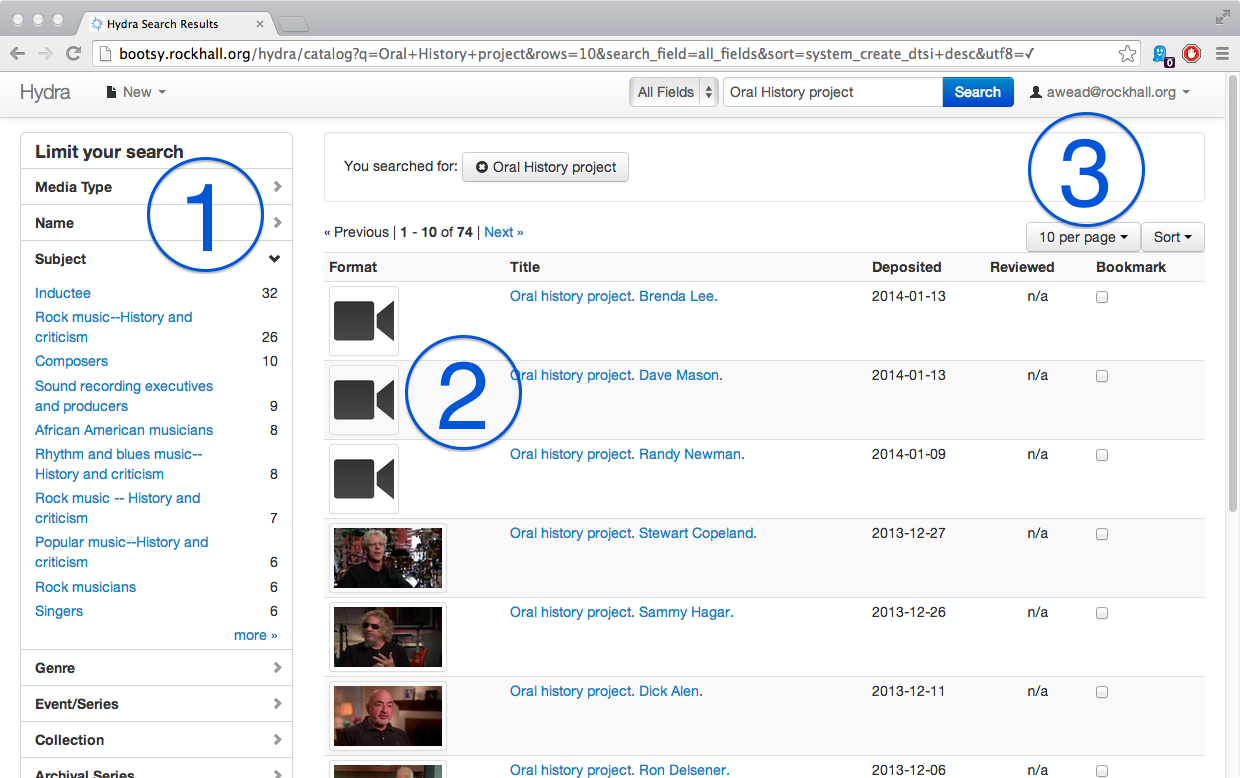
\includegraphics[height=10em]{images/search}}
    \end{multicols}
  }

  \headerbox{Editing}{name=edit,column=0,span=2,below=overview}{
    \begin{multicols}{2}
      \noindent{Users can edit titles, subjects, and permissions, as well as
      metadata for each derivative. Records are externally linked to finding aids
      by selecting collections and series headings (2) taken from Archivist's Toolkit.
      Users can view each file's technical metadata or download access copies (3).}
      \noindent{\centering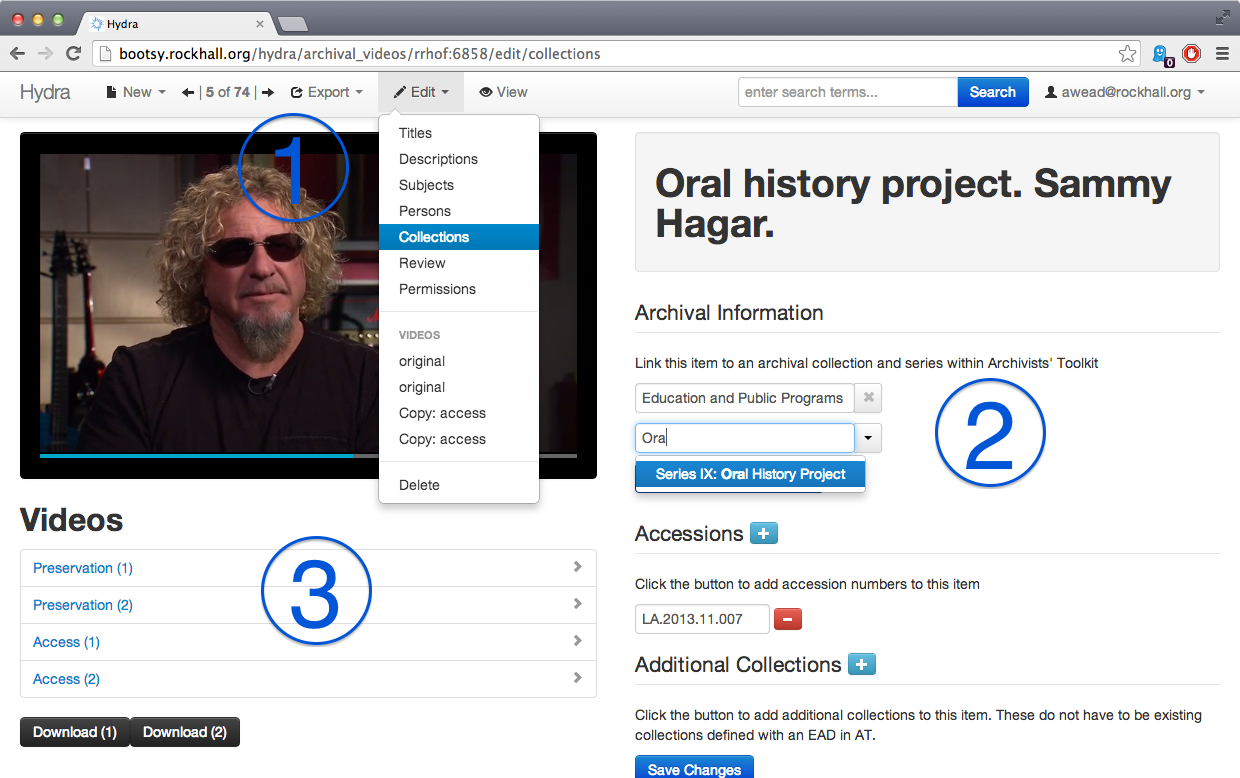
\includegraphics[height=10em]{images/edit}}
    \end{multicols}
  }

  \headerbox{Detailed Display}{name=show,column=0,span=2,below=edit}{
    \begin{multicols}{2}
      \noindent{The detailed show view of a video includes playback controls (1).
      A complete item record (2) shows all of the 
      descriptive metadata for the video such as title, subject headings, and
      a summary.  The technical metadata for the first video segment (3) is
      expanded to show some of the fields.  This metadata is gathered at ingest
      using MediaInfo.}
      \noindent{\centering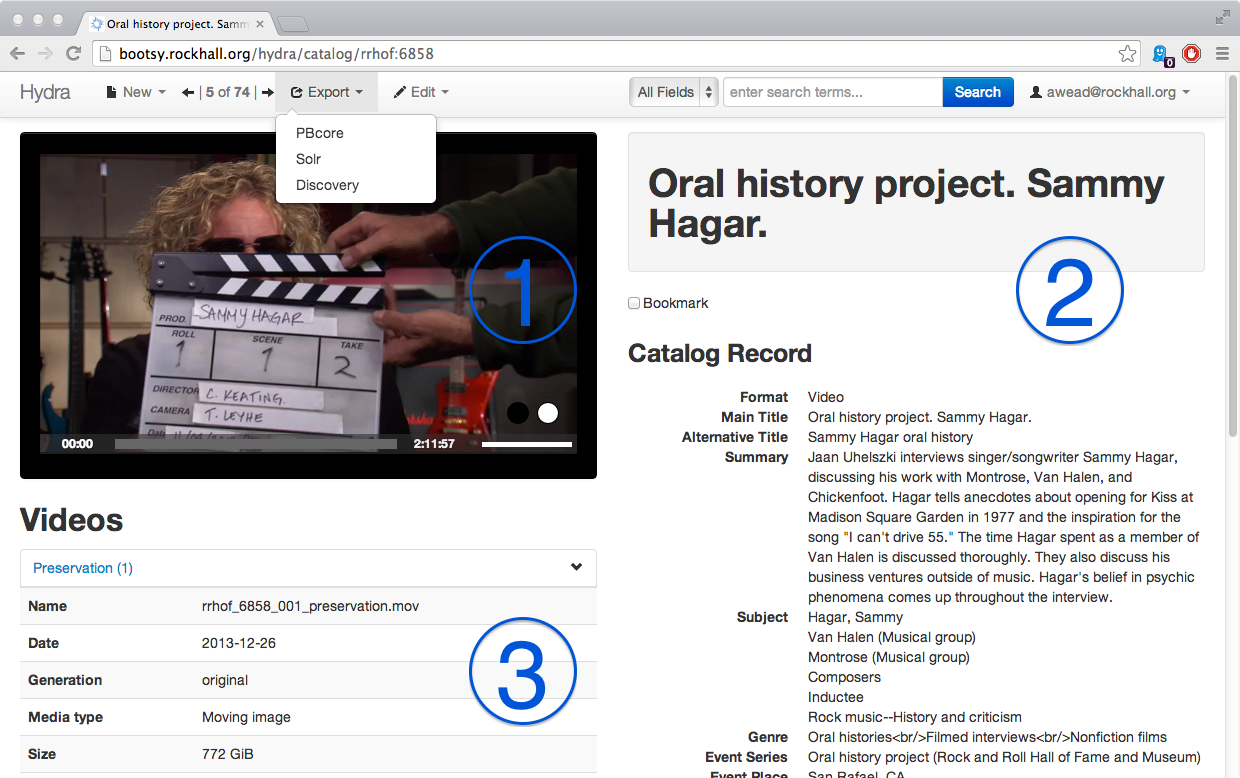
\includegraphics[height=10em]{images/show}}
    \end{multicols}
  }

  \headerbox{Discovery}{name=discover,column=2,below=search}{
    \noindent{Content is exported for discovery
    using a Blacklight application with marc and ead data, as well
    as the exported PBCore records from Hydra.  The video shown below
    is displayed within the context of its finding aid.  Users
    can navigate the breadcrumb trail back through the current series (2) 
    or view other parts of the 
    finding aid and the rest of its inventory (1).
    The descriptive metadata (3) and the video come from
    Hydra.}
    \noindent{\centering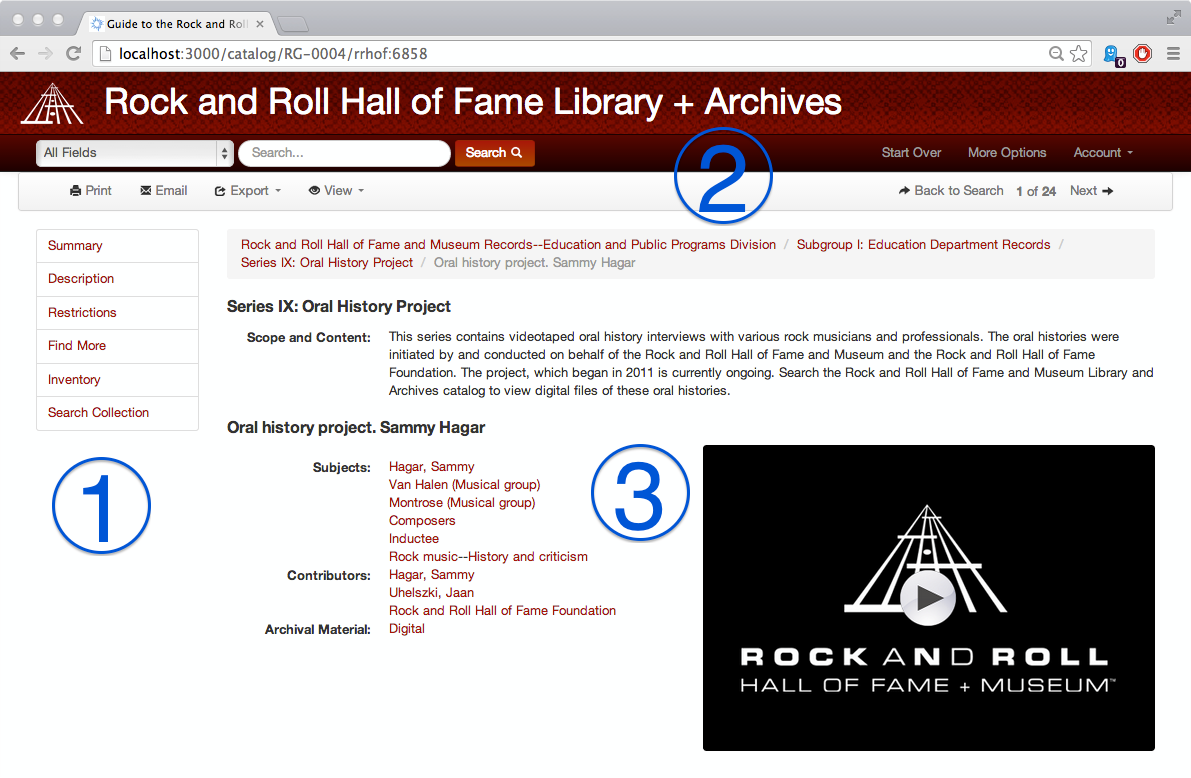
\includegraphics[height=10em]{images/discover}}
  }



\end{poster}

\end{document}
